As described in \secref{intro_motivation}, deep networks suffer from early commitment.
However, the \emph{Gestalt} psychology \cite{ellis_source_1938, kohler_gestalt_1992, wagemans_century_2012, hamlyn_psychology_2017}, as well as the theory of natural intelligence \cite{von_der_malsburg_theory_2022} and work based on self-organising projection fibres (c.f. \secref{projection_fibres}) considers the principle of preventing early commitment as a core mechanism for the effectiveness of the human visual system.

The human brain can prevent early commitment while still being an excellent image-processing system. 
Consequently, the neuroscientific literature is studied, and promising findings to implement a vision framework preventing early commitment are identified.
Thus, this chapter can be considered a survey of existing neuroscientific findings.
However, compared to the related work section, it contains more interpretations and introduces a unified vocabulary compatible with both fields, neuroscience and deep learning.

In the following, \secref{neuroscience_findings} presents important neuroscientific findings, describing lateral connections (\secref{neuroscience_findings_lateral_connections}), net fragments (\secref{neuroscience_findings_net_fragments}), the local learning principle (\secref{neuroscience_findings_local_learning_principle}), and projection fibres (\secref{neuroscience_findings_projection_fibres}).
Finally, \secref{biologial_inspiration_vision} describes the vision of how these biological findings could improve current systems.



\section{Neuroscientific Findings}\seclbl{neuroscience_findings}

\subsection{The Brain's Visual System}
\begin{figure}[h]
    \centering
    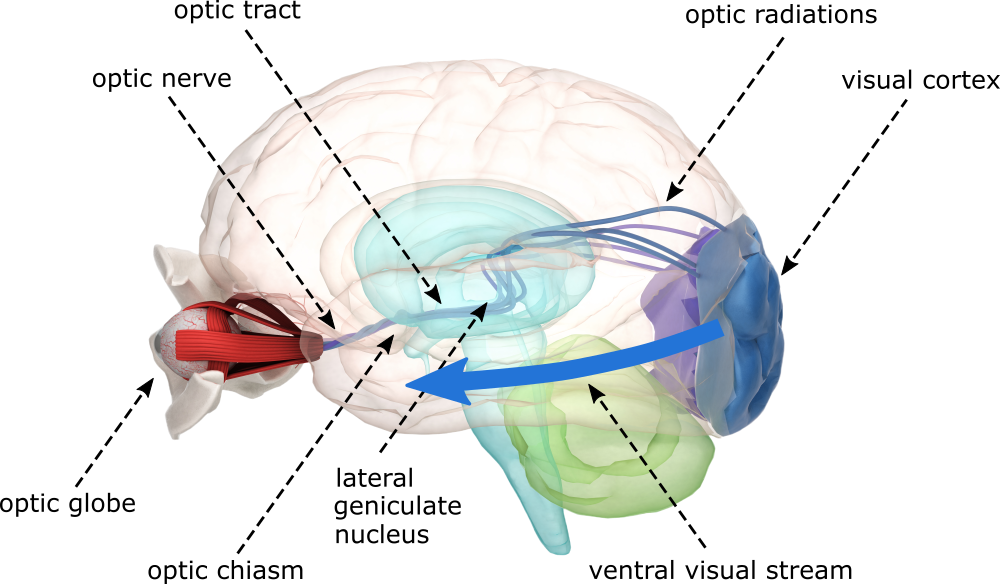
\includegraphics[width=0.99\textwidth]{Visual-System}
    \caption[Visualisation of the human's visual system]{Visualisation of the human's visual system. The image is from \citeay{fasoli_human_2023}.}
    \figlbl{visual_system}
\end{figure}
%
The visual system of humans is visualised in \figref{visual_system}. The eyes function as sensors that capture light waves and translate them into electrical pulses. This electrical signal travels through the human brain to the primary visual cortex \sidecite{tong_primary_2003, grill-spector_human_2004}, located at the back of the head.
Cells within the visual cortex fire spikes when specific visual stimuli appear within their receptive fields. Thus, these cells can be considered filters that are excited if a known pattern is detected in the input data. 

However, the visual cortex only detects patterns in visual data but does not draw conclusions from it. Instead, it forwards it as an information stream to other brain areas. In this thesis, especially the ventral visual stream is of importance. This stream forwards the detected patterns to the temporal cortex \sidecite{miyashita_inferior_1993, conway_organization_2018}, a brain region located behind the ears.
According to the two-stream hypothesis \sidecite{goodale_separate_1992}, the temporal cortex is responsible for object identification and recognition. A second stream, the dorsal stream, forwards the same data to the parietal cortex, a region on top of the head that predicts the object's spatial location relative to the viewer \sidecite{colby_space_1999}. However, this stream is of less importance in this thesis.

The brain implements this behaviour using net fragments, lateral connections, and projection fibres. These fundamental elements of the brain serve as inspiration for the proposed framework and are introduced in the following.

\begin{figure}[h]
    \centering
    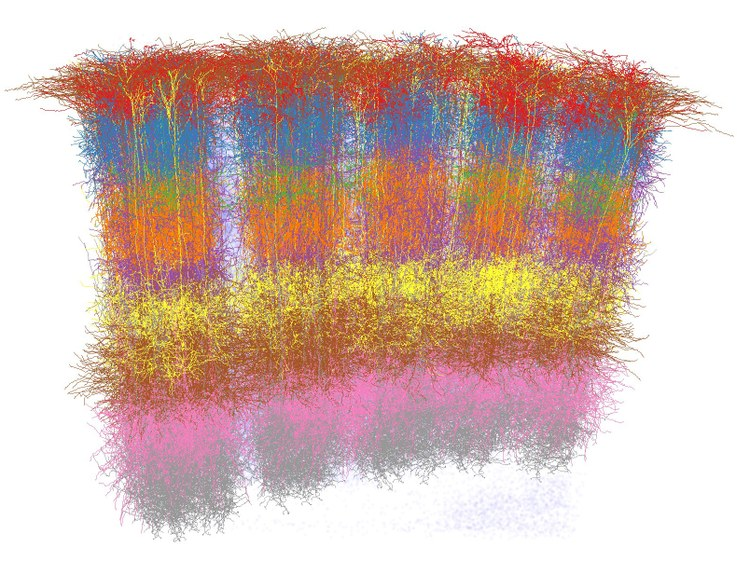
\includegraphics[width=0.99\textwidth]{cortical_columns}
    \caption[3D reconstruction of five neighbouring cortical columns]{3D reconstruction of five neighboring cortical columns of a rat. The image is from \citeay{oberlaender_beyond_2012}.}
    \figlbl{cortical_columns}
\end{figure}

\subsection{Lateral Connections and Lateral Support}\seclbl{neuroscience_findings_lateral_connections}
The cerebral cortex forms the outer hull of the brain \cite{narr_relationships_2007} and encompasses several regions, including the previously mentioned visual and temporal cortex, as well as the ventral visual stream.
The cerebral cortex consists of many cylindrical arrangements of neurons called cortical columns \sidecite{mountcastle_columnar_1997}.
A 3D reconstruction of five cortical columns is shown in \figref{cortical_columns}, with different layers visualised by different colours.

Information in the cerebral cortex is propagated forward from one layer to the next and has inspired layer-wise processing in deep learning architectures \sidecite{prince_understanding_2023}.
However, a closer look at the human brain reveals that there are also connections between neurons within the same layer that process information locally \sidecite{gilbert_lateral_1990}.
These intra-layer connections are called \emph{lateral connections} and are visualised in a simplified manner in \figref{lateral_connections} for a single neuron.
Notably, such a neuron not only establishes connections to neurons in the preceding and subsequent layers (marked in orange and green) but also lateral connections to neurons within its own layer (marked in red).

\begin{figure}[h]
    \centering
    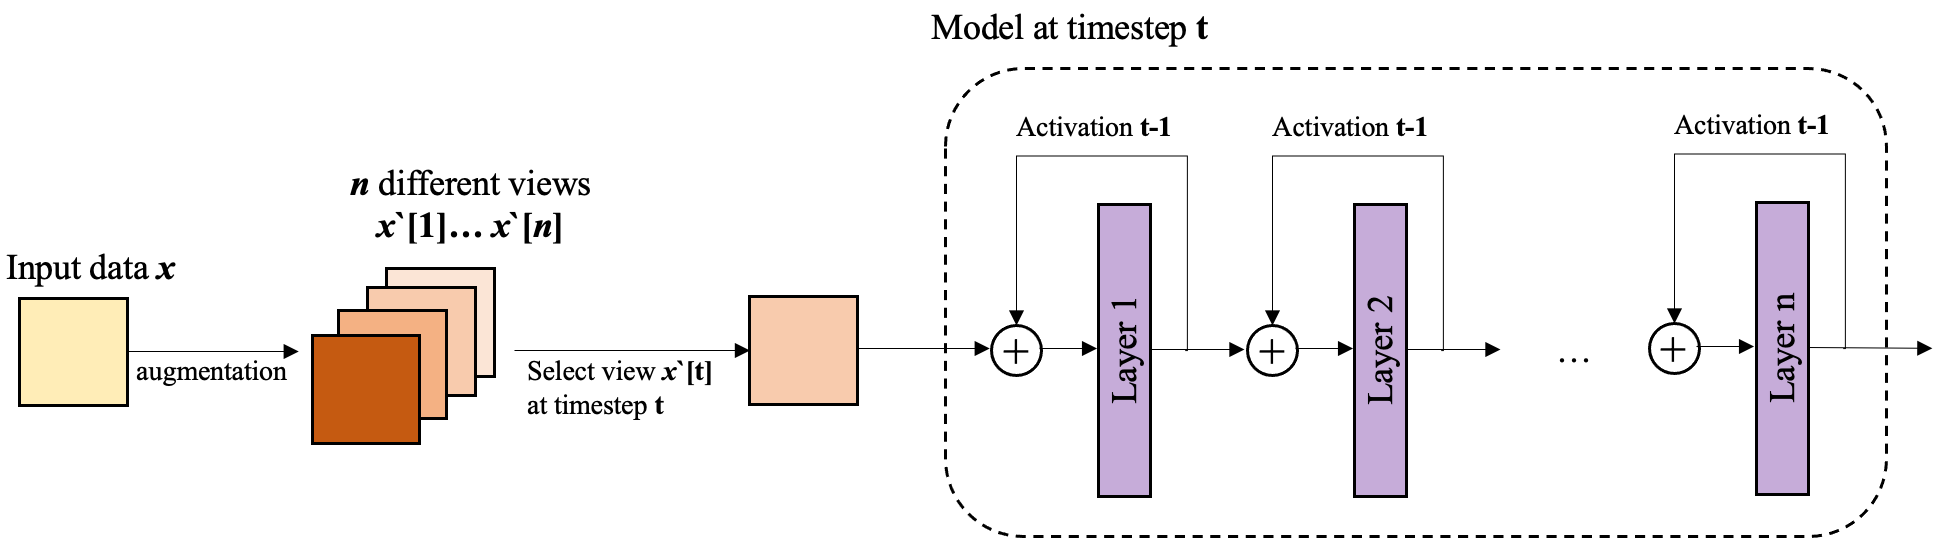
\includegraphics[width=0.99\textwidth]{lateral_connections}
    \caption[Lateral connections of a cell]{Visualisation of the connections of a single cell. The cell is connected to the previous layer (orange), the subsequent layer (green), and to neurons within the same layer (lateral connections, red).}
    \figlbl{lateral_connections}
\end{figure}

According to \sideciteay{von_der_malsburg_theory_2022}, these lateral connections are used for \emph{lateral support}. ``Lateral support'' means that neurons from the same layer support each other's activity:
Neurons from the preceding layer can activate the red cell in \figref{lateral_connections} through the orange connections.
However, inhibitory signals can suppress the activity of the red neuron before it has a chance to fire a spike to the subsequent layer via the green connections. The neuron can only transmit a spike to the subsequent layers if it ``survives'' an inhibition phase \cite{coombs_specific_1955}, which is only possible if it receives sufficient lateral support from laterally connected neurons.
Suppose the preceding layer activates several neurons within the same layer as the red neuron, and these activated neurons exhibit lateral connections. In that case, they can send spikes to each other, thereby providing mutual support. This allows them to maintain their action potential and remain active during the inhibition phase.

\subsection{Net Fragments}\seclbl{neuroscience_findings_net_fragments}
Lateral connections grow between cells that are often active together \sidecite{hebb_organization_1949}.
Since cells are often active together when they represent the same pattern, this increases lateral support between groups of neurons representing frequently occurring patterns. Such groups are called \emph{net fragments}.
All neurons within a net fragment support each other to remain active during an inhibition phase. 
Thus, a layer with multiple net fragments can be considered a filter: While the previous layer might activate numerous cells, only the cells with sufficient lateral support remain active. Therefore, only learned patterns survive and send a spike to the next layer.

\subsubsection{Local Neighbourhood}
\begin{figure}[h]
    \centering
    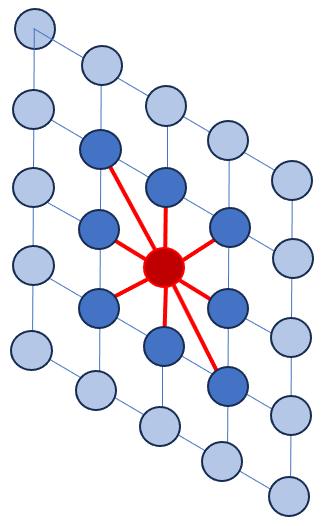
\includegraphics[width=0.4\textwidth]{local_neighbourhood2}
    \caption[Lateral connections limited to a local neighbourhood]{The lateral connections limited to a local neighbourhood.}
    \figlbl{local_neighbourhood2}
\end{figure}
Net fragments represent patterns that can be distinguished between local patterns, which are spatially limited to a local area, and global patterns, which extend over larger regions of the image and might encompass the entire image.
The number of possible patterns increases exponentially with the size of the considered patterns. Thus, local patterns occur more frequently.
In order to learn frequently occurring patterns, the range of the lateral connections must be limited to a \emph{local neighbourhood}, similar to convolutional filters (c.f. \secref{cnns}).
Capturing global patterns would require exponentially more cells than if local patterns are captured. Therefore, limiting the range of lateral connections to local neighbourhoods is crucial.
\figref{local_neighbourhood2} illustrates such limited lateral connections: The lateral connections from the red cell do not encompass the entire image but are only connected to cells that are in close proximity.

The size of the local neighbourhood in the human brain varies \sidecite{pessoa_understanding_2014}.
The primary visual cortex captures the input signal with a high local variance and therefore has a strongly limited local neighbourhood size. The temporal cortex contains transformation-independent object representations and can afford larger neighbourhood sizes as fewer distinct global patterns exist.

\subsubsection{Hierarchy of Net Fragments}
A single cell is supported by its neighbouring cells, which, in turn, are supported by their neighbouring cells. Therefore, the support reaches much further than only the local neighbourhood.
As the processing progresses, increasing inhibition causes cells without sufficient support to be turned off. Turning off one cell can trigger a chain reaction of further turn-offs. Therefore, lateral support occurs not only between individual cells but also between many overlapping net fragments.

Thus, the network consists of a hierarchy of net fragments, which can be interpreted as a larger net fragment, i.e. a multitude of cells supporting each other.
The size of a net fragment cannot be defined; the smallest possible net fragment is a single cell with its local neighbourhood, while the largest net fragment can span all active cells that are laterally connected.

\subsubsection{Alternative Cells and Pathways}\seclbl{neuroscience_findings_alt_cells}
In a given spatial location, different patterns can occur.
However, the capacity of a net fragment is limited to represent a single pattern.
For example, cell $A$ may often fire with cells $B$ and $C$ in close proximity, exhibiting a high mutual lateral support with these cells.
However, cells $B$ and $C$ might not fire together. Consequently, cell $A$ is involved in two distinct and mutually exclusive net fragments, once together with cell $B$ and once with cell $C$.
To facilitate such coexistence between net fragments, \emph{alternative cells} are required. A copy of cell $A$ must exist that behaves similarly but has different synaptic connections, i.e. exhibits \emph{alternative pathways}.
The precise biological mechanism of how this is implemented is unclear; One hypothesis is that within a group of cells that initially have similar afferent connections, cells undergo divergent connectivity changes during training, resulting in cells specialising in different patterns. This process allows to split a cell at the same spatial location and enables the formation of alternative and mutually exclusive net fragments.

\subsection{Local Learning Principle}\seclbl{neuroscience_findings_local_learning_principle}
In the brain, consistency is evaluated at the level of individual synapses in every single point in the network \sidecite{hebb_organization_1949}. Each synapse is established if the firing of its source neuron and its target neuron are consistent, allowing the source neuron to predict the activity of the target neuron. This process is crucial for establishing net structures, where each neuron within a net fragment can predict the firing of other neurons with a high probability.
This local learning is a key difference between natural (animal or human) learning and the frequently used backpropagation of error \sidecite{rosenblatt_principles_1962, linnainmaa_taylor_1976}. With backpropagation, consistency is optimised at a single point, specifically between the system's output and a teacher signal. All synapses, including those that are distantly connected (the ``deep'' connections), are guided by the consistency of this single point. Therefore, the human brain is dominated by local learning and self-organisation, while deep networks typically use a global learning rule that guides the learning process of the entire network.


\subsection{Projection Fibres}\seclbl{neuroscience_findings_projection_fibres}
\begin{figure}[h]
    \centering
    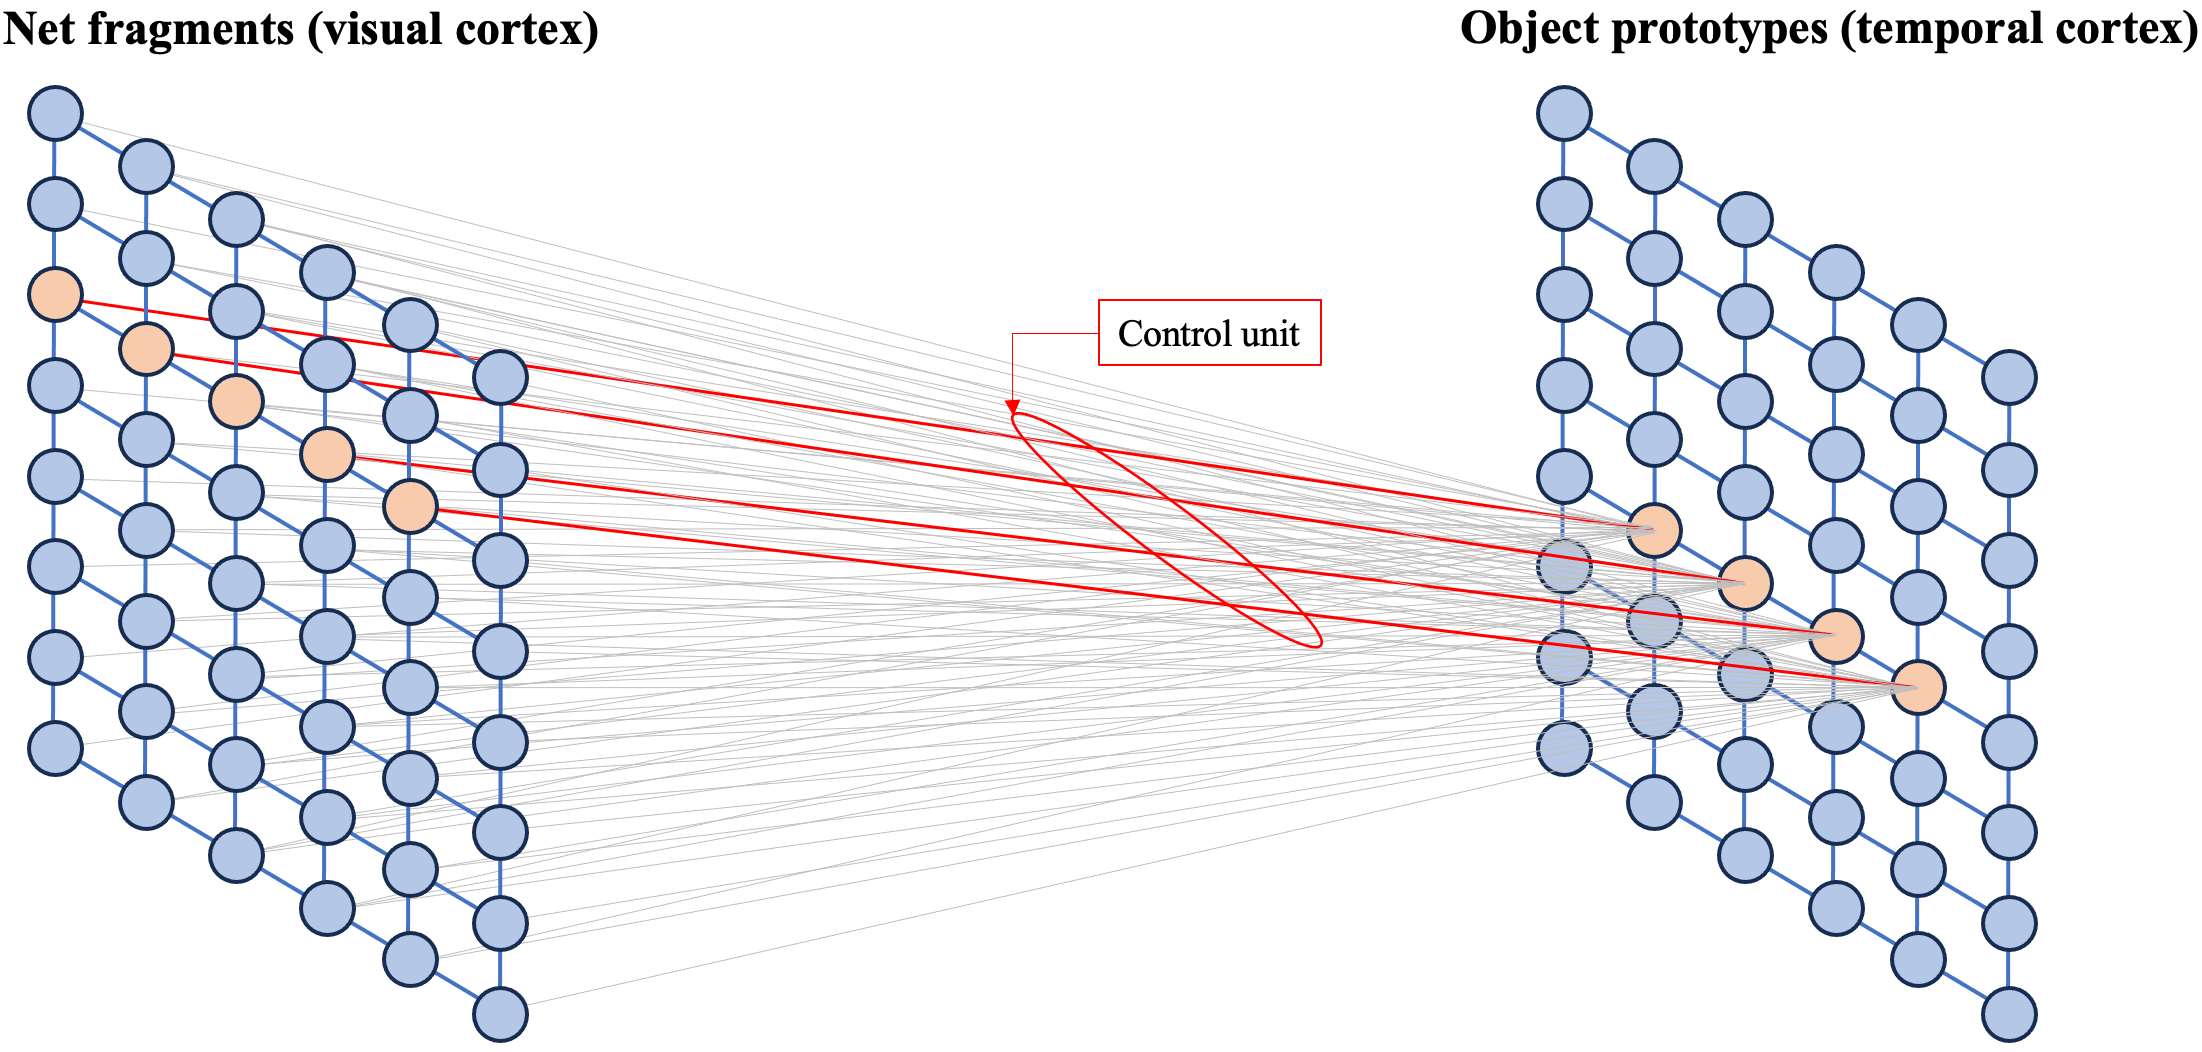
\includegraphics[width=0.99\textwidth]{maplets}
    \caption[An active maplet mapping net fragments to object prototypes]{Net fragments (on the left) are projected to an object (on the right). Many projection fibres (grey) run between the net fragments and objects, but only a few of them belonging to the same maplet (red) have been turned on.}
    \figlbl{maplets}
\end{figure}
%
As described at the beginning of this chapter, the visual cortex extracts pattern from visual information. This process is implemented with the aforementioned building blocks, such as lateral connections and net fragments. In theory, this is sufficient to implement the principles from the Gestalt psychology \cite{ellis_source_1938, kohler_gestalt_1992, wagemans_century_2012, hamlyn_psychology_2017}. However, it is not sufficient for efficient visual object detection.

In the human brain, object detection takes place in the temporal cortex, a region that is spatially distant from the visual cortex.
The brain's solution to transmit information over such long distances are \emph{projection fibres} (axons) \sidecite{greig_molecular_2013}.
Projection fibres are links between neurons in the visual cortex and object prototypes (so-called reference frames) in the temporal cortex.

Object prototypes in the temporal cortex are net fragments similar to those in the visual cortex. However, the fragments in the visual cortex are an overlay of multiple fragments between cells activated by the eyes.
This overlay of fragments is a description of a captured visual scene, whereby it is unclear which sub-fragments represent distinct objects and how they are related.
On the other hand, the fragments in the temporal cortex depict exactly one single object, whereby these objects are position and transformation-invariant.

Projection fibres map neurons within the captured scene (in the primary visual cortex) to object prototypes (in the temporal cortex) with one-to-one connections \sidecite{anderson_shifter_1987}, where pairs of neurons connected in the visual cortex project to pairs of neurons connected in the temporal cortex. The projection fibres have some flexibility, allowing for local distortions and enabling transformation- and position-invariant mapping \sidecite{wolfrum_recurrent_2008, wiskott_face_1996}. This mapping allows the recognition of one or more objects in a scene and their relationships to each other, facilitating object recognition and scene interpretation.

\subsubsection{Maplets and Control Units}
Each existing neuron in the visual cortex has projection fibres running to the temporal cortex. Consequently, there is a multitude of projection fibres, but only a fraction are active at any given time.
Typically, the same set of projection fibres is activated by similar patterns.
Such sets of projection fibres that are activated at the same time are grouped into \emph{maplets} \sidecite{zhu_maplets_2004}.
\emph{Control units} decide which maplets are activated and thus initiate the mapping between the visual and temporal cortex. 
A control unit in the human brain is a unipolar neuron, a kind of neuron with extensions (so-called processes) that end in synapses and can conduct signals in both directions - from the synapse to the neuron and from the neuron to the synapse \sidecite{byrne_oxford_2019}.
Control units trigger a mapping when a net fragment in the visual cortex matches well another fragment in the temporal cortex, i.e. when these two fragments have a high correlation. However, they only remain active if numerous other projection fibres confirm the decision and map their respective fragments in the visual cortex to the same object prototype. By doing so, the human brain generates numerous hypotheses about observations, but inhibitory signals quickly deactivate most projections, leaving only the plausible ones active.

\figref{maplets} visualises such a projection between net fragments and an object prototype of a line. A vast amount of projection fibres (grey) run between these two areas, but only the most suitable ones are activated by the control unit of a maplet (red).
Please note that the line on the left is translated and stretched. However, the projection fibres still map such a transformed object to an idealised prototype.
\figref{maplets} shows a direct mapping from net fragments to prototypes for better clarity. However, this mapping is done in the brain over several hierarchical levels, saving many projection fibres \sidecite{anderson_shifter_1987}.

Projection fibres thus provide generalisation, i.e. different, transformed versions of an object are recognised and mapped to a reference frame. This explains the ability of humans to see a new object once and immediately recognise it in a transformed version.

\section{Objective}\seclbl{biologial_inspiration_vision}
The aforementioned neuroscientific findings serve as the foundation to build a novel image-processing framework.
The core behind this framework is based on two stages and projection fibres connecting them.
The first stage builds net fragments reassembling a visual scene captured with a sensory system (the eyes). The lateral reach within this stage is limited since many pattern combinations can be experienced in the real world. However, scenes are dominated by locally similar-looking patterns that can be captured with net fragments.
The second stage contains not entire visual scenes but reference frames representing specific objects. These objects are centred and transformation-invariant and can thus afford longer-reaching lateral connections.
Multiple 2D reference frames must exist for each object to represent an object from various viewpoints.

Projection fibres connect these two stages, mapping objects within a visual scene to object prototypes.
This mapping serves as a scene interpretation layer by describing which objects are located where in the observed scene.
In the next \chref{probabilistic_framework}, a framework is proposed that implements these two stages with projection fibres.
It is considered a computational implementation of the foundation of the biological visual system.
However, in the long term, this framework can be further expanded and is not limited to these two stages, thereby leading to a highly efficient scene processing system.
These extensions are discussed in the following.

\subsection{Object Classification}
A classification layer maps an object to a specific instance, for example, a person, to a person's name. Projection fibres do not provide such a classification as these fibres map the pattern to a more generalised view, i.e. transforming a person to a reference person. Instead, a subsequent memory stage is needed to map a reference object to an actual label.
This memory stage contains multiple instances for each object and provides distinction between objects. The memory stage implements an n-to-n mapping to the reference frame: Each reference frame has multiple instances (e.g. multiple persons exist), and each instance can belong to multiple reference frames (e.g. a face and a body could be different reference frames but belong to the same instance).

The human brain has cells representing instances of objects \sidecite{gross_genealogy_2002}.
Therefore, memory is assumed to consist of one or a few cells, while reference frames consist of many cells.
This allows to store many object instances while not requiring a vast number of cells.


\subsection{Scene Interpretation}
On a very abstract level, I envision the mapping process as having a big canvas with the observed visual scene in the middle and arrows going away from each object in the image and pointing to the corresponding prototype. Thus, the projection fibres (the arrows) implement object segmentation and identification.
In addition, the position of each object is known, as well as the differences in position between the objects.
Such a canvas provides a mental description of a perceived scene. However, such a description is not sufficient to interpret a scene. For scene interpretation, all objects in the scene must be put into context.

As described in \secref{neuroscience_findings_local_learning_principle}, the human brain optimises consistency at every point in the network: Consistency is optimised between the cells within the two stages to build net fragments and between the projection fibres connection net fragments to obtain a valid mapping.
However, building consistency between these two stages is not enough to interpret visual scenes.

In the long term, more components must be added, allowing to build consistency between memories and reference frames.
For instance, projection fibres could map one object in the scene to a person while mapping another object in close spatial proximity of this person's foot to a ball. By building consistency between these two objects, one could conclude that this person is most likely playing football (soccer). Synaptic connections between these references could be formed if such scenes are observed several times, allowing for scene interpretation.
Furthermore, memories could be integrated that either confirms or rejects this hypothesis. If, for example, the person is identified as a soccer player such as Ronaldo, it would further strengthen this hypothesis.

Such a system could learn interpretations of visual scenes and might even have the potential to understand how objects are related to each other. A pivotal difference to deep networks is that the model can build such consistency on its own, while deep learning systems require a teaching signal to learn consistency.
I speculate that having a system that can build consistency of completely unseen scenes without teaching signals might be a step towards emergence.


\subsection{Preventing Early Commitment}\seclbl{biologial_inspiration_early_commitment}
As described in the previous section, deep learning models are prone to early commitment \sidecite{marr_vision_2010}.
The brain's solution to prevent early commitment are net fragments.
A single layer with lateral connections that forms net fragments can represent local and global features at the same time\sidenote{This way of thinking about features can be hard to comprehend, especially for computer scientists familiar with deep learning.}.
Each set of active and laterally connected neurons can be considered a net fragment. Net fragments with a few cells depict local features, while fragments containing many features represent more global features.

A system that avoids the fallacy of early commitment should solve the conundrum that local decisions are taken based on plausibility in the light of high-level patterns, while high-level patterns can only be defined based on low-level features.
The most fundamental local decision is whether a single cell should be active. Since a single cell receives support from all laterally connected cells, a high-level pattern (i.e. the activity of all directly or indirectly laterally connected cells) is used to make this decision. Therefore, local decisions are taken based on high-level patterns. The high-level pattern used to make this decision is defined by the sum of individual cells (i.e. low-level features). Hence, the human brain solves the conundrum within every single layer.


\subsection{Hierarchical Features}
Neuroscientific findings indicate that the human brain does not rely on a sequence of layers to build feature hierarchies as often done in deep networks.
In the biological context, layers have other connotations, and evidence suggests that layers in cortical columns deal with depth rotations \sidecite{iamshchinina_perceived_2021}.
In the proposed framework, feature hierarchies are implicitly stored in net fragments whereby a larger fragment represents a more global feature, and smaller fragments have more local features.
Consequently, sequences of layers are not necessary to represent feature hierarchies.

However, multiple stages are required to build abstractions of input signals, i.e. to generalise features.
In the human brain, several regions interact with each other to generate abstractions \sidecite{felleman_distributed_1991}.
In fact, the visual cortex builds net fragments based on the signal from the eyes, projection fibres map the object to prototypes, and other fibres map the prototypes to memories and interpret them. Thus, various stages are involved in processing images.
Furthermore, processing takes place over a short amount of time until all stages reach a consensus. Thus, no layer-wise processing is required as in deep, but multiple stages interact with each other to build feature abstractions.

